\section{Conception de la classe Station d'alimentation}
\label{sec:stationAlimentation}

\begin{center}
    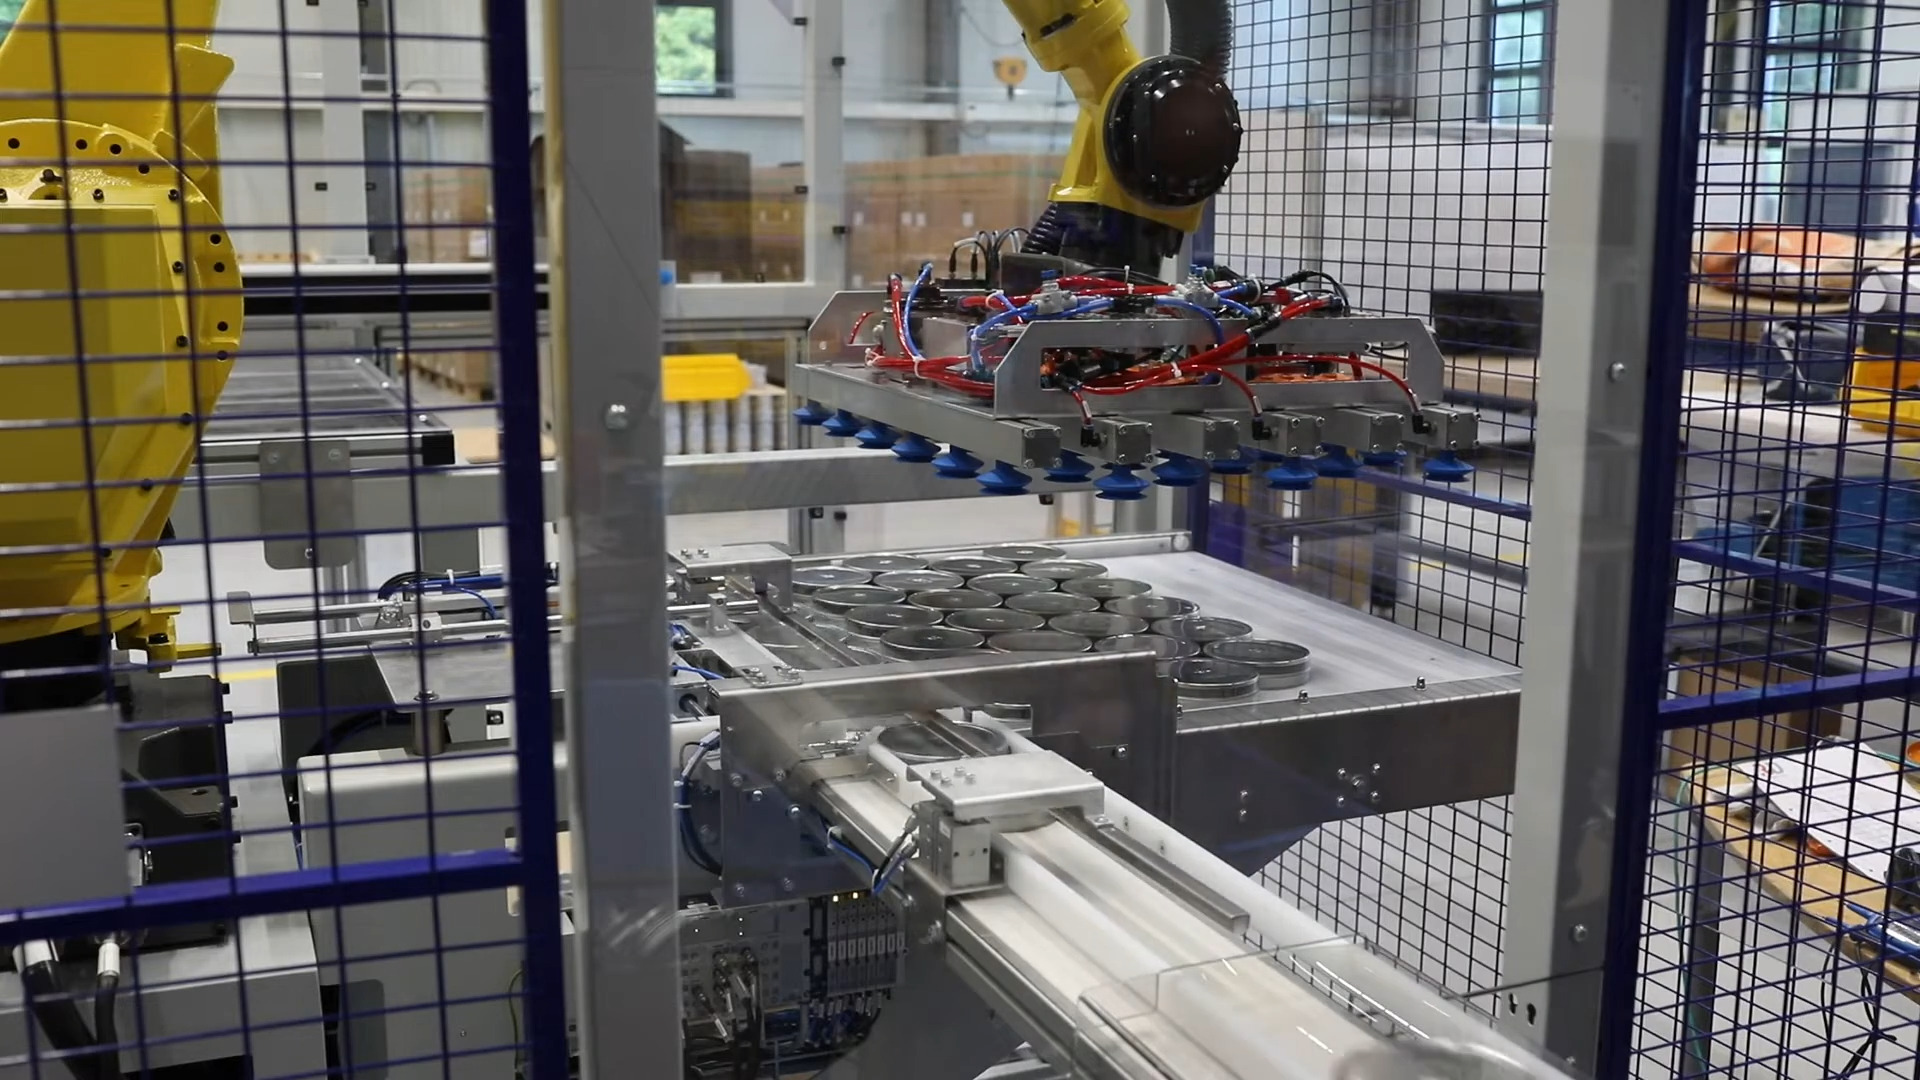
\includegraphics[width=0.7\textwidth]{figures/remplissageTampon}
\end{center}

La station d'alimentation est responsable de la préparation des boîtes de conserve en vue de leur palettisation. Les boîtes arrivent sur un convoyeur horizontal. A l'entrée du poste, un capteur permet de compter le nombre de boîtes afin de former des lots de 6 unités. Chaque lot est ensuite poussé perpendiculairement vers une zone tampon, rangée après rangée, jusqu'à former une couche complète.

Un système de butée mobile permet de décaler horizontalement la position finale de chaque rangée, formant ainsi une disposition en quinconce. Ce principe assure la stabilité des couches pour la suite du processus de palettisation.

\begin{center}
    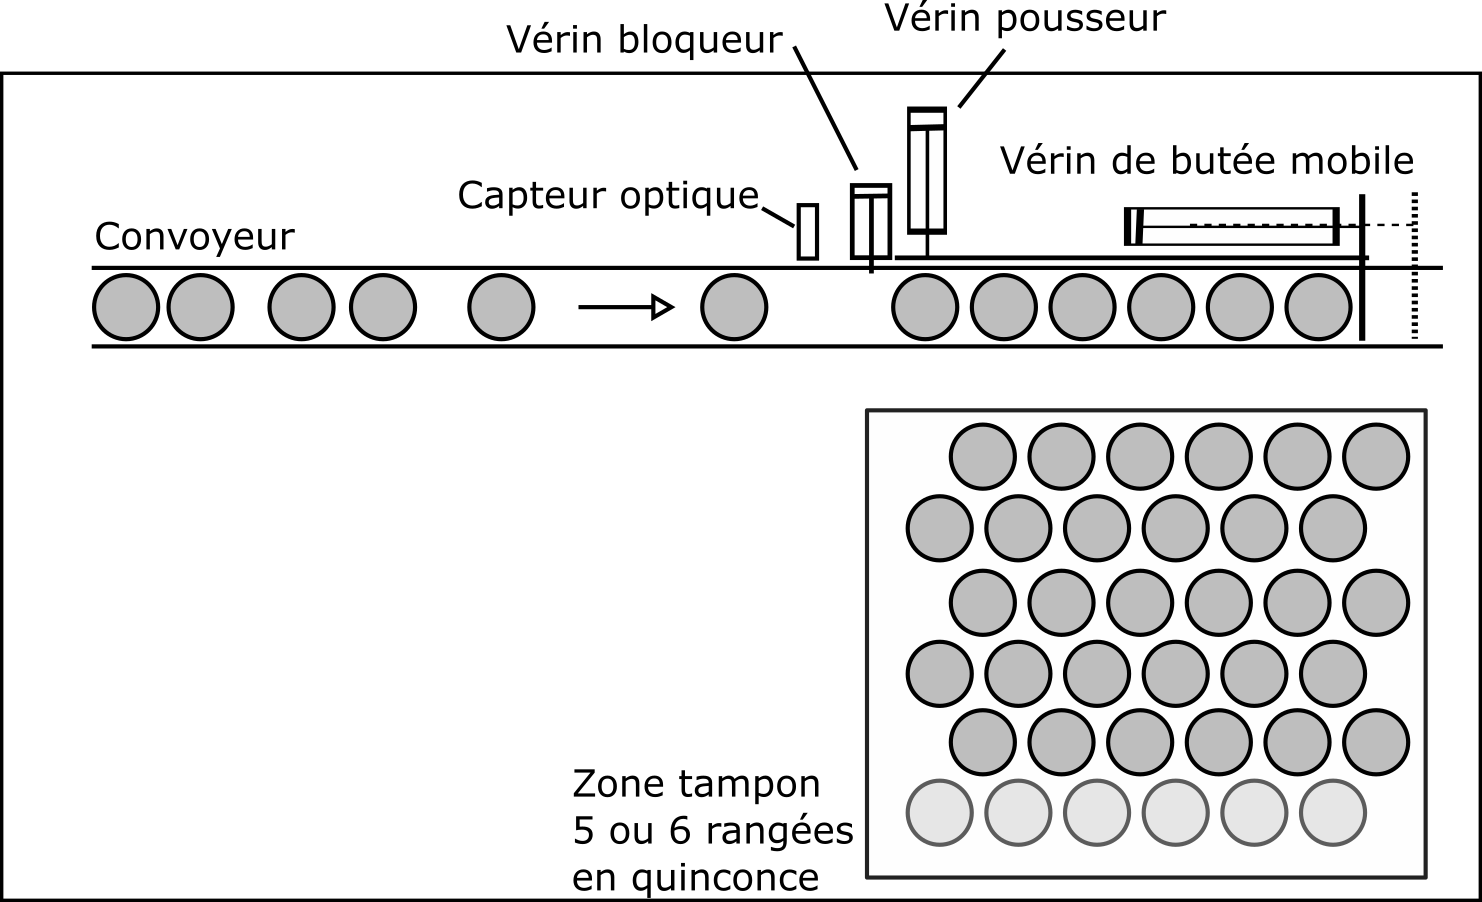
\includegraphics[width=0.7\textwidth]{figures/station_alimentation.png}
\end{center}

\paragraph{Actionneurs}
\begin{itemize}
    \item \textbf{Convoyeur motorisé} : transporte les boîtes depuis l'entrée de la station jusqu'à la zone de regroupement. Fonctionne en continu.
    \item \textbf{Vérin de butée mobile :} placé dans le sens du convoyeur, il agit comme une butée réglable. En position rentrée, il bloque les boîtes plus tôt. En position sortie, il les laisse avancer plus loin. L'alternance de ces deux positions permet de former des rangées en quinconce. Il s'agit d'un vérin double effet, commandé par un distributeur mono-stable.
    \item \textbf{Vérin pousseur} : placé perpendiculairement au convoyeur, il pousse chaque lot de 6 boîtes dans la zone tampon. Il s'agit d'un vérin simple effet, commandé par un distributeur mono-stable.
    \item \textbf{Un vérin bloqueur} : placé à l'entrée de la zone tampon, il empèche le passage des boîtes lorsque la zone d'attente est pleine. 
\end{itemize}

\paragraph{Capteurs}
\begin{itemize}
    \item \textbf{Capteur inductif de comptage} : détecte le passage de chaque boîte pour compter exactement 6 boîtes par lot.
    \item \textbf{Capteurs de fin de course du vérin pousseur} : détectent les positions extrêmes du vérin. 
    \item \textbf{Capteurs de fin de course du vérin de butée} : indique si la butée est en position rentrée ou sortie.
\end{itemize}

\paragraph{Remarques}
\begin{itemize}
    \item Une couche est constituée de 5 à 6 rangées de 6 boîtes.
\end{itemize}
